% Capítulo 2
\chapter{Insertion Sort}

\section{Gráficos}
\subsection{Melhor caso}
O gráfico abaixo representa o tempo de execução do melhor caso do insertion-sort em função do tamanho da entrada. Como entrada para gerar o gráfico, foram utilizados 91 vetores já ordenados. Pela análise do gráfico podemos notar que o algoritmo no melhor caso, desconsiderando a variação de tempo gerada por processos concorrentes no momento da execução do programa, é linear. Tb(n) pertence a O(n).
\begin{figure}[h]
    \centering
    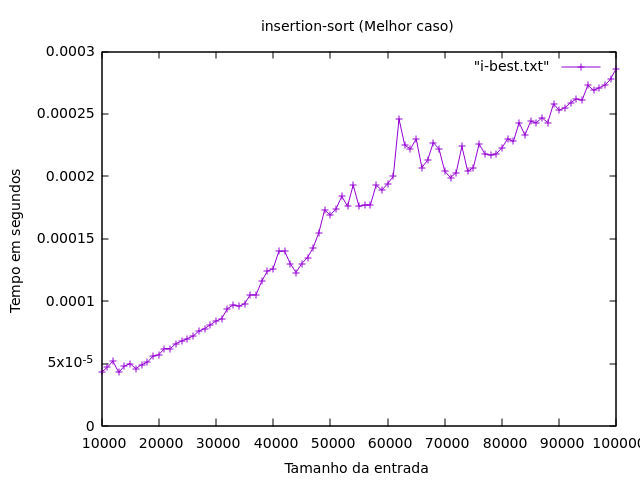
\includegraphics[width=1\linewidth]{Imagens/i-best.png}
\end{figure}

\newpage

\subsection{Pior caso}
O gráfico abaixo representa o tempo de execução do pior caso do insertion-sort em função do tamanho da entrada. Como entrada para gerar o gráfico, foram utilizados 91 vetores ordenados em ordem decrescente. Pela análise do gráfico podemos notar que o algoritmo no pior caso, desconsiderando a variação de tempo gerada por processos concorrentes no momento da execução do programa, é quadrático. Tw(n) pertence a O(n²).
\begin{figure}[h]
    \centering
    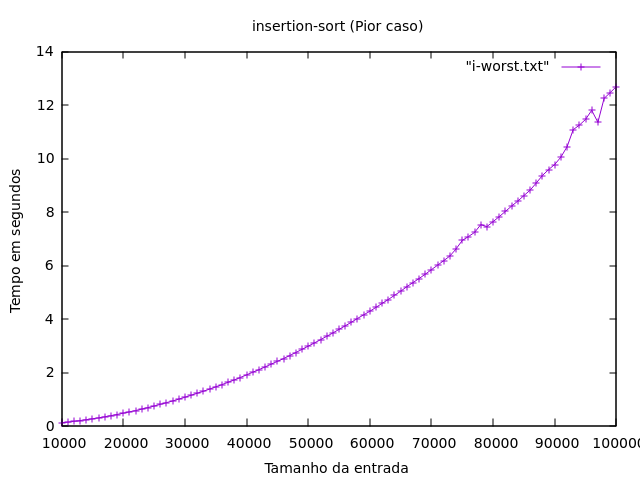
\includegraphics[width=1\linewidth]{Imagens/i-worst.png}
\end{figure}

\newpage

\subsection{Caso médio}
O gráfico abaixo representa o tempo de execução esperado do insertion-sort em função do tamanho da entrada. Como entrada para gerar o gráfico, foram utilizados 91 vetores de tamanho n, preenchidos com números de 0 até n gerados aleatoriamente. Pela análise do gráfico podemos notar que o algoritmo no caso médio, desconsiderando a variação de tempo gerada por processos concorrentes no momento da execução do programa, é quadrático. Ta(n) pertence a O(n²).
\begin{figure}[h]
    \centering
    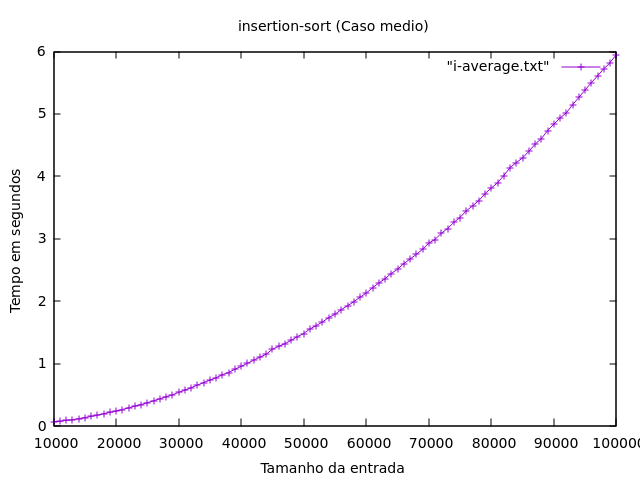
\includegraphics[width=1\linewidth]{Imagens/i-average.png}
\end{figure}

\newpage

\subsection{Comparação dos gráficos}
No gráfico abaixo podemos ver a comparação entre o caso médio, o melhor e o pior caso do algoritmo.
\begin{figure}[h]
    \centering
    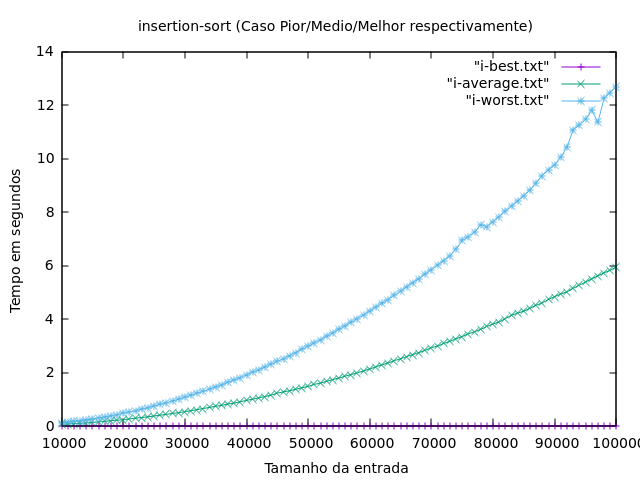
\includegraphics[width=1\linewidth]{Imagens/i-baw.png}
\end{figure}

\newpage

\section{Análise analítica do tempo de execução}

\subsection{Algoritmo}
\begin{figure}[h]
    \centering
    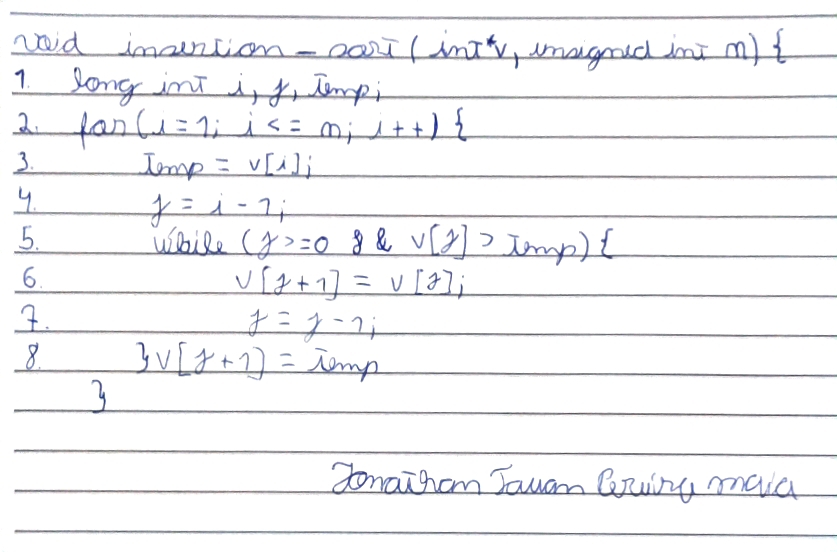
\includegraphics[width=0.76\linewidth]{Imagens/insertion.jpg}
\end{figure}

\newpage

\subsubsection{Melhor caso}
A análise analítica do tempo de execução do insertion-sort no melhor caso, que se dá quando o vetor de entrada já está ordenado, permitiu perceber novamente que este é da forma linear, f(n) = an + b.
\begin{figure}[h]
    \centering
    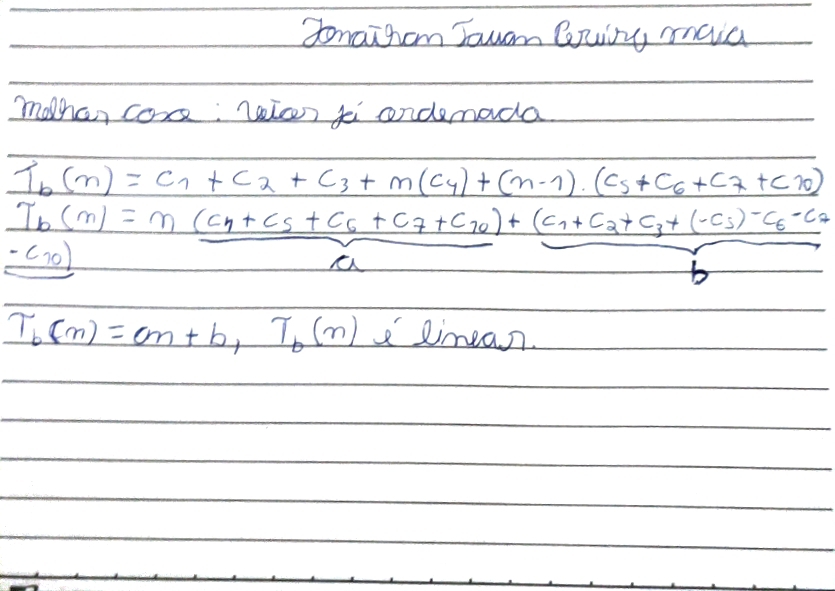
\includegraphics[width=0.76\linewidth]{Imagens/melhor-insertion.jpg}
\end{figure}

\newpage

\subsubsection{Pior caso}
A análise analítica do tempo de execução do insertion-sort no pior caso, que se dá quando o vetor de entrada está ordenado em ordem decrescente, permitiu perceber também que este é da forma quadrática, f(n) = an² +
bn + c.
\begin{figure}[h]
    \centering
    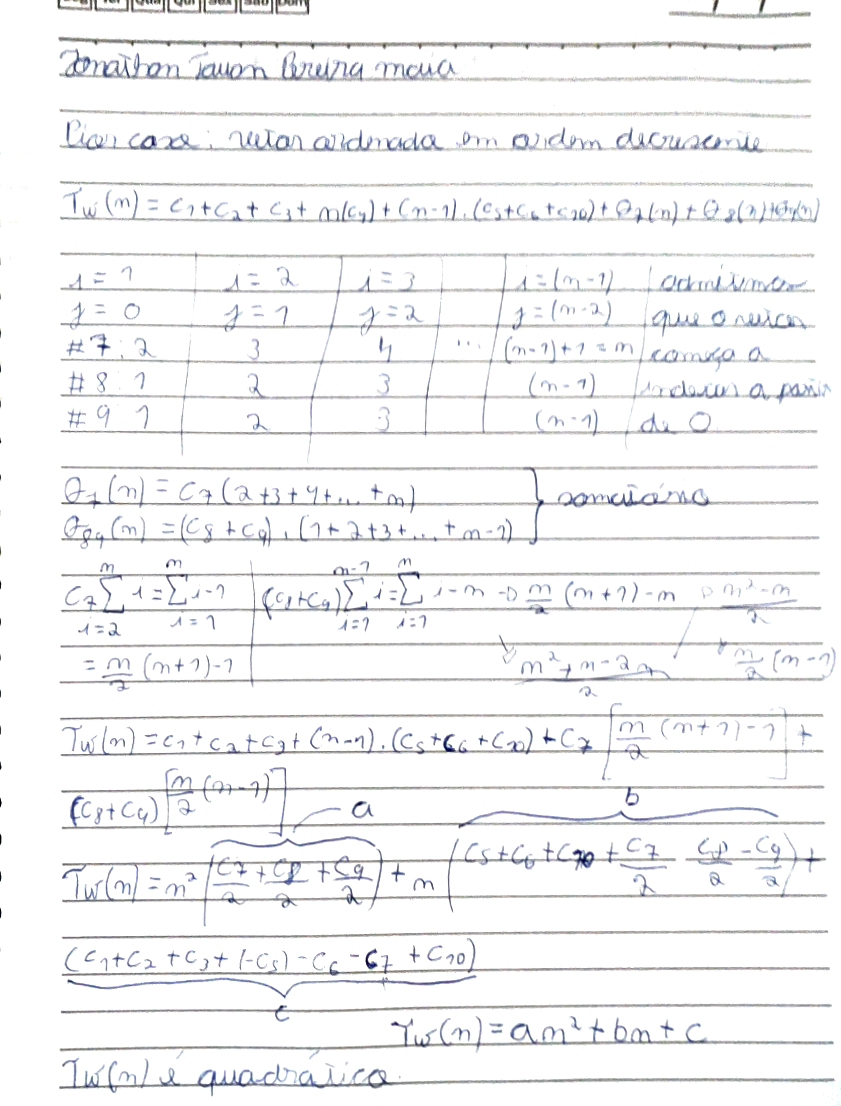
\includegraphics[width=0.76\linewidth]{Imagens/pior-insertion.jpg}
\end{figure}
